\documentclass[1p]{elsarticle_modified}
%\bibliographystyle{elsarticle-num}

%\usepackage[colorlinks]{hyperref}
%\usepackage{abbrmath_seonhwa} %\Abb, \Ascr, \Acal ,\Abf, \Afrak
\usepackage{amsfonts}
\usepackage{amssymb}
\usepackage{amsmath}
\usepackage{amsthm}
\usepackage{scalefnt}
\usepackage{amsbsy}
\usepackage{kotex}
\usepackage{caption}
\usepackage{subfig}
\usepackage{color}
\usepackage{graphicx}
\usepackage{xcolor} %% white, black, red, green, blue, cyan, magenta, yellow
\usepackage{float}
\usepackage{setspace}
\usepackage{hyperref}

\usepackage{tikz}
\usetikzlibrary{arrows}

\usepackage{multirow}
\usepackage{array} % fixed length table
\usepackage{hhline}

%%%%%%%%%%%%%%%%%%%%%
\makeatletter
\renewcommand*\env@matrix[1][\arraystretch]{%
	\edef\arraystretch{#1}%
	\hskip -\arraycolsep
	\let\@ifnextchar\new@ifnextchar
	\array{*\c@MaxMatrixCols c}}
\makeatother %https://tex.stackexchange.com/questions/14071/how-can-i-increase-the-line-spacing-in-a-matrix
%%%%%%%%%%%%%%%

\usepackage[normalem]{ulem}

\newcommand{\msout}[1]{\ifmmode\text{\sout{\ensuremath{#1}}}\else\sout{#1}\fi}
%SOURCE: \msout is \stkout macro in https://tex.stackexchange.com/questions/20609/strikeout-in-math-mode

\newcommand{\cancel}[1]{
	\ifmmode
	{\color{red}\msout{#1}}
	\else
	{\color{red}\sout{#1}}
	\fi
}

\newcommand{\add}[1]{
	{\color{blue}\uwave{#1}}
}

\newcommand{\replace}[2]{
	\ifmmode
	{\color{red}\msout{#1}}{\color{blue}\uwave{#2}}
	\else
	{\color{red}\sout{#1}}{\color{blue}\uwave{#2}}
	\fi
}

\newcommand{\Sol}{\mathcal{S}} %segment
\newcommand{\D}{D} %diagram
\newcommand{\A}{\mathcal{A}} %arc


%%%%%%%%%%%%%%%%%%%%%%%%%%%%%5 test

\def\sl{\operatorname{\textup{SL}}(2,\Cbb)}
\def\psl{\operatorname{\textup{PSL}}(2,\Cbb)}
\def\quan{\mkern 1mu \triangleright \mkern 1mu}

\theoremstyle{definition}
\newtheorem{thm}{Theorem}[section]
\newtheorem{prop}[thm]{Proposition}
\newtheorem{lem}[thm]{Lemma}
\newtheorem{ques}[thm]{Question}
\newtheorem{cor}[thm]{Corollary}
\newtheorem{defn}[thm]{Definition}
\newtheorem{exam}[thm]{Example}
\newtheorem{rmk}[thm]{Remark}
\newtheorem{alg}[thm]{Algorithm}

\newcommand{\I}{\sqrt{-1}}
\begin{document}

%\begin{frontmatter}
%
%\title{Boundary parabolic representations of knots up to 8 crossings}
%
%%% Group authors per affiliation:
%\author{Yunhi Cho} 
%\address{Department of Mathematics, University of Seoul, Seoul, Korea}
%\ead{yhcho@uos.ac.kr}
%
%
%\author{Seonhwa Kim} %\fnref{s_kim}}
%\address{Center for Geometry and Physics, Institute for Basic Science, Pohang, 37673, Korea}
%\ead{ryeona17@ibs.re.kr}
%
%\author{Hyuk Kim}
%\address{Department of Mathematical Sciences, Seoul National University, Seoul 08826, Korea}
%\ead{hyukkim@snu.ac.kr}
%
%\author{Seokbeom Yoon}
%\address{Department of Mathematical Sciences, Seoul National University, Seoul, 08826,  Korea}
%\ead{sbyoon15@snu.ac.kr}
%
%\begin{abstract}
%We find all boundary parabolic representation of knots up to 8 crossings.
%
%\end{abstract}
%\begin{keyword}
%    \MSC[2010] 57M25 
%\end{keyword}
%
%\end{frontmatter}

%\linenumbers
%\tableofcontents
%
\newcommand\colored[1]{\textcolor{white}{\rule[-0.35ex]{0.8em}{1.4ex}}\kern-0.8em\color{red} #1}%
%\newcommand\colored[1]{\textcolor{white}{ #1}\kern-2.17ex	\textcolor{white}{ #1}\kern-1.81ex	\textcolor{white}{ #1}\kern-2.15ex\color{red}#1	}

{\Large $\underline{11n_{134}~(K11n_{134})}$}

\setlength{\tabcolsep}{10pt}
\renewcommand{\arraystretch}{1.6}
\vspace{1cm}\begin{tabular}{m{100pt}>{\centering\arraybackslash}m{274pt}}
\multirow{5}{120pt}{
	\centering
	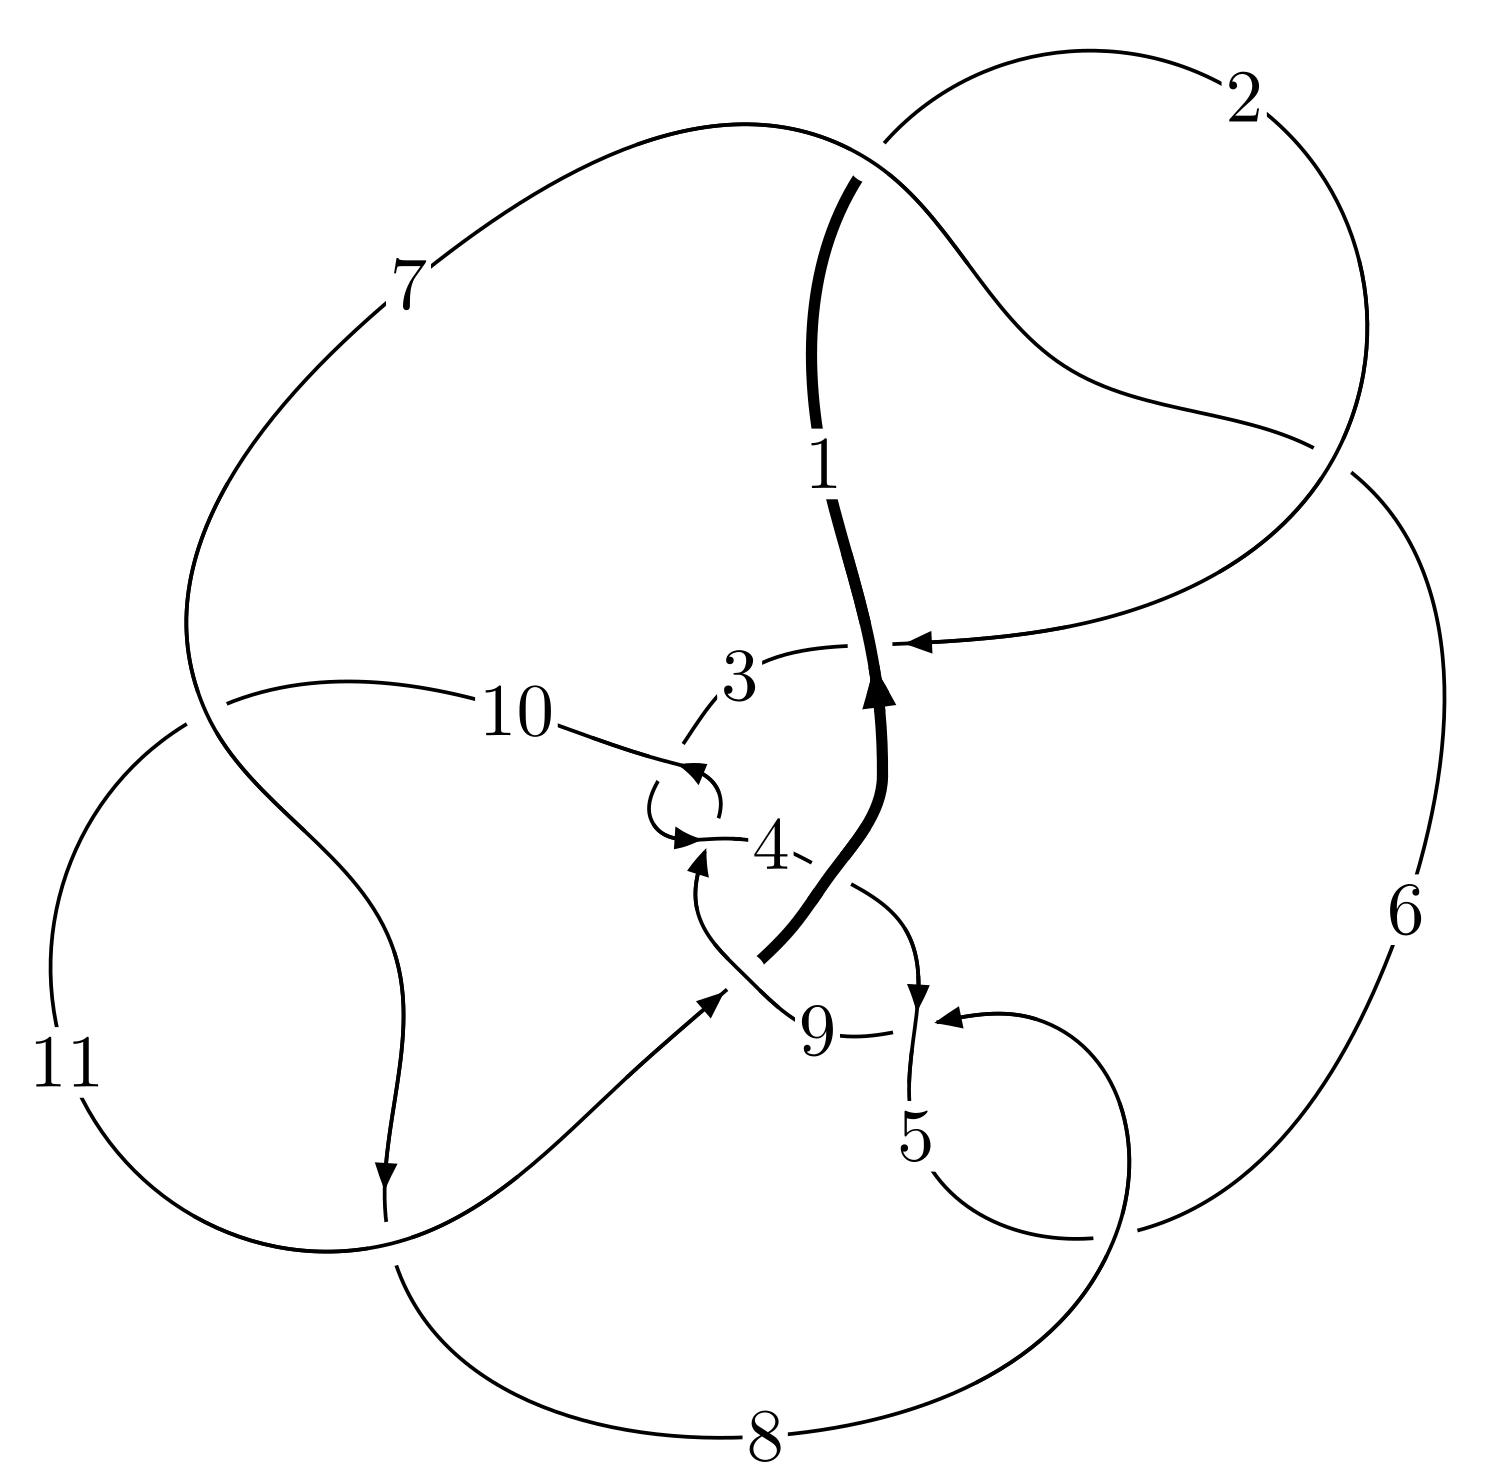
\includegraphics[width=112pt]{../../../GIT/diagram.site/Diagrams/png/750_11n_134.png}\\
\ \ \ A knot diagram\footnotemark}&
\allowdisplaybreaks
\textbf{Linearized knot diagam} \\
\cline{2-2}
 &
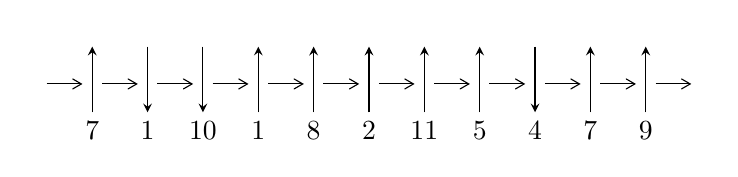
\begin{tikzpicture}[x=20pt, y=17pt]
	% nodes
	\node (C0) at (0, 0) {};
	\node (C1) at (1, 0) {};
	\node (C1U) at (1, +1) {};
	\node (C1D) at (1, -1) {7};

	\node (C2) at (2, 0) {};
	\node (C2U) at (2, +1) {};
	\node (C2D) at (2, -1) {1};

	\node (C3) at (3, 0) {};
	\node (C3U) at (3, +1) {};
	\node (C3D) at (3, -1) {10};

	\node (C4) at (4, 0) {};
	\node (C4U) at (4, +1) {};
	\node (C4D) at (4, -1) {1};

	\node (C5) at (5, 0) {};
	\node (C5U) at (5, +1) {};
	\node (C5D) at (5, -1) {8};

	\node (C6) at (6, 0) {};
	\node (C6U) at (6, +1) {};
	\node (C6D) at (6, -1) {2};

	\node (C7) at (7, 0) {};
	\node (C7U) at (7, +1) {};
	\node (C7D) at (7, -1) {11};

	\node (C8) at (8, 0) {};
	\node (C8U) at (8, +1) {};
	\node (C8D) at (8, -1) {5};

	\node (C9) at (9, 0) {};
	\node (C9U) at (9, +1) {};
	\node (C9D) at (9, -1) {4};

	\node (C10) at (10, 0) {};
	\node (C10U) at (10, +1) {};
	\node (C10D) at (10, -1) {7};

	\node (C11) at (11, 0) {};
	\node (C11U) at (11, +1) {};
	\node (C11D) at (11, -1) {9};
	\node (C12) at (12, 0) {};

	% arrows
	\draw[->,>={angle 60}]
	(C0) edge (C1) (C1) edge (C2) (C2) edge (C3) (C3) edge (C4) (C4) edge (C5) (C5) edge (C6) (C6) edge (C7) (C7) edge (C8) (C8) edge (C9) (C9) edge (C10) (C10) edge (C11) (C11) edge (C12) ;	\draw[->,>=stealth]
	(C1D) edge (C1U) (C2U) edge (C2D) (C3U) edge (C3D) (C4D) edge (C4U) (C5D) edge (C5U) (C6D) edge (C6U) (C7D) edge (C7U) (C8D) edge (C8U) (C9U) edge (C9D) (C10D) edge (C10U) (C11D) edge (C11U) ;
	\end{tikzpicture} \\
\hhline{~~} \\& 
\textbf{Solving Sequence} \\ \cline{2-2} 
 &
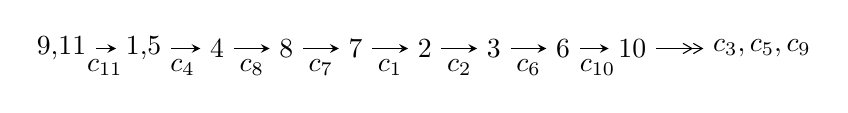
\begin{tikzpicture}[x=25pt, y=7pt]
	% node
	\node (A0) at (-1/8, 0) {9,11};
	\node (A1) at (17/16, 0) {1,5};
	\node (A2) at (17/8, 0) {4};
	\node (A3) at (25/8, 0) {8};
	\node (A4) at (33/8, 0) {7};
	\node (A5) at (41/8, 0) {2};
	\node (A6) at (49/8, 0) {3};
	\node (A7) at (57/8, 0) {6};
	\node (A8) at (65/8, 0) {10};
	\node (C1) at (1/2, -1) {$c_{11}$};
	\node (C2) at (13/8, -1) {$c_{4}$};
	\node (C3) at (21/8, -1) {$c_{8}$};
	\node (C4) at (29/8, -1) {$c_{7}$};
	\node (C5) at (37/8, -1) {$c_{1}$};
	\node (C6) at (45/8, -1) {$c_{2}$};
	\node (C7) at (53/8, -1) {$c_{6}$};
	\node (C8) at (61/8, -1) {$c_{10}$};
	\node (A9) at (10, 0) {$c_{3},c_{5},c_{9}$};

	% edge
	\draw[->,>=stealth]	
	(A0) edge (A1) (A1) edge (A2) (A2) edge (A3) (A3) edge (A4) (A4) edge (A5) (A5) edge (A6) (A6) edge (A7) (A7) edge (A8) ;
	\draw[->>,>={angle 60}]	
	(A8) edge (A9);
\end{tikzpicture} \\ 

\end{tabular} \\

\footnotetext{
The image of knot diagram is generated by the software ``\textbf{Draw programme}" developed by Andrew Bartholomew(\url{http://www.layer8.co.uk/maths/draw/index.htm\#Running-draw}), where we modified some parts for our purpose(\url{https://github.com/CATsTAILs/LinksPainter}).
}\phantom \\ \newline 
\centering \textbf{Ideals for irreducible components\footnotemark of $X_{\text{par}}$} 
 
\begin{align*}
I^u_{1}&=\langle 
9.34789\times10^{32} u^{33}-5.58712\times10^{32} u^{32}+\cdots+1.57006\times10^{31} b-1.59332\times10^{33},\\
\phantom{I^u_{1}}&\phantom{= \langle  }3.16774\times10^{33} u^{33}-1.98307\times10^{33} u^{32}+\cdots+1.57006\times10^{31} a-4.97227\times10^{33},\;u^{34}-4 u^{32}+\cdots-8 u-1\rangle \\
I^u_{2}&=\langle 
2 u^6- u^5-3 u^4+6 u^3+2 u^2+b-6 u+2,\;3 u^6- u^5-4 u^4+9 u^3+4 u^2+a-7 u+3,\\
\phantom{I^u_{2}}&\phantom{= \langle  }u^7- u^6- u^5+4 u^4- u^3-3 u^2+3 u-1\rangle \\
I^u_{3}&=\langle 
u^2+b- u-1,\;- u^2+a+2 u-1,\;u^4-2 u^3+u+1\rangle \\
\\
\end{align*}
\raggedright * 3 irreducible components of $\dim_{\mathbb{C}}=0$, with total 45 representations.\\
\footnotetext{All coefficients of polynomials are rational numbers. But the coefficients are sometimes approximated in decimal forms when there is not enough margin.}
\newpage
\renewcommand{\arraystretch}{1}
\centering \section*{I. $I^u_{1}= \langle 9.35\times10^{32} u^{33}-5.59\times10^{32} u^{32}+\cdots+1.57\times10^{31} b-1.59\times10^{33},\;3.17\times10^{33} u^{33}-1.98\times10^{33} u^{32}+\cdots+1.57\times10^{31} a-4.97\times10^{33},\;u^{34}-4 u^{32}+\cdots-8 u-1 \rangle$}
\flushleft \textbf{(i) Arc colorings}\\
\begin{tabular}{m{7pt} m{180pt} m{7pt} m{180pt} }
\flushright $a_{9}=$&$\begin{pmatrix}0\\u\end{pmatrix}$ \\
\flushright $a_{11}=$&$\begin{pmatrix}1\\0\end{pmatrix}$ \\
\flushright $a_{1}=$&$\begin{pmatrix}1\\- u^2\end{pmatrix}$ \\
\flushright $a_{5}=$&$\begin{pmatrix}-201.759 u^{33}+126.306 u^{32}+\cdots+2044.63 u+316.694\\-59.5386 u^{33}+35.5855 u^{32}+\cdots+631.913 u+101.482\end{pmatrix}$ \\
\flushright $a_{4}=$&$\begin{pmatrix}-64.0473 u^{33}+42.6334 u^{32}+\cdots+604.027 u+88.9064\\-110.441 u^{33}+66.5690 u^{32}+\cdots+1163.58 u+185.154\end{pmatrix}$ \\
\flushright $a_{8}=$&$\begin{pmatrix}126.520 u^{33}-77.8350 u^{32}+\cdots-1331.80 u-221.282\\144.062 u^{33}-89.2523 u^{32}+\cdots-1486.79 u-232.342\end{pmatrix}$ \\
\flushright $a_{7}=$&$\begin{pmatrix}-17.5420 u^{33}+11.4173 u^{32}+\cdots+154.996 u+11.0598\\144.062 u^{33}-89.2523 u^{32}+\cdots-1486.79 u-232.342\end{pmatrix}$ \\
\flushright $a_{2}=$&$\begin{pmatrix}191.791 u^{33}-115.291 u^{32}+\cdots-2025.26 u-313.383\\-1.17243 u^{33}+1.47552 u^{32}+\cdots+5.92933 u+1.12007\end{pmatrix}$ \\
\flushright $a_{3}=$&$\begin{pmatrix}123.827 u^{33}-75.2327 u^{32}+\cdots-1300.65 u-199.211\\22.2954 u^{33}-12.2052 u^{32}+\cdots-246.576 u-38.9385\end{pmatrix}$ \\
\flushright $a_{6}=$&$\begin{pmatrix}-403.100 u^{33}+247.007 u^{32}+\cdots+4184.10 u+645.587\\-156.172 u^{33}+97.4389 u^{32}+\cdots+1597.51 u+249.393\end{pmatrix}$ \\
\flushright $a_{10}=$&$\begin{pmatrix}-68.1247 u^{33}+44.5777 u^{32}+\cdots+659.086 u+90.0150\\28.9676 u^{33}-18.5354 u^{32}+\cdots-294.427 u-45.6978\end{pmatrix}$\\ \flushright $a_{10}=$&$\begin{pmatrix}-68.1247 u^{33}+44.5777 u^{32}+\cdots+659.086 u+90.0150\\28.9676 u^{33}-18.5354 u^{32}+\cdots-294.427 u-45.6978\end{pmatrix}$\\&\end{tabular}
\flushleft \textbf{(ii) Obstruction class $= -1$}\\~\\
\flushleft \textbf{(iii) Cusp Shapes $= 263.563 u^{33}-150.065 u^{32}+\cdots-2900.73 u-454.146$}\\~\\
\newpage\renewcommand{\arraystretch}{1}
\flushleft \textbf{(iv) u-Polynomials at the component}\newline \\
\begin{tabular}{m{50pt}|m{274pt}}
Crossings & \hspace{64pt}u-Polynomials at each crossing \\
\hline $$\begin{aligned}c_{1},c_{6}\end{aligned}$$&$\begin{aligned}
&u^{34}+u^{33}+\cdots-223 u+11
\end{aligned}$\\
\hline $$\begin{aligned}c_{2}\end{aligned}$$&$\begin{aligned}
&u^{34}+39 u^{33}+\cdots-30545 u+121
\end{aligned}$\\
\hline $$\begin{aligned}c_{3},c_{9}\end{aligned}$$&$\begin{aligned}
&u^{34}+2 u^{32}+\cdots-30 u+11
\end{aligned}$\\
\hline $$\begin{aligned}c_{4}\end{aligned}$$&$\begin{aligned}
&u^{34}+6 u^{33}+\cdots+88 u-16
\end{aligned}$\\
\hline $$\begin{aligned}c_{5},c_{8}\end{aligned}$$&$\begin{aligned}
&u^{34}+3 u^{33}+\cdots+73 u+11
\end{aligned}$\\
\hline $$\begin{aligned}c_{7},c_{10}\end{aligned}$$&$\begin{aligned}
&u^{34}- u^{33}+\cdots-33 u-1
\end{aligned}$\\
\hline $$\begin{aligned}c_{11}\end{aligned}$$&$\begin{aligned}
&u^{34}-4 u^{32}+\cdots-8 u-1
\end{aligned}$\\
\hline
\end{tabular}\\~\\
\newpage\renewcommand{\arraystretch}{1}
\flushleft \textbf{(v) Riley Polynomials at the component}\newline \\
\begin{tabular}{m{50pt}|m{274pt}}
Crossings & \hspace{64pt}Riley Polynomials at each crossing \\
\hline $$\begin{aligned}c_{1},c_{6}\end{aligned}$$&$\begin{aligned}
&y^{34}+39 y^{33}+\cdots-30545 y+121
\end{aligned}$\\
\hline $$\begin{aligned}c_{2}\end{aligned}$$&$\begin{aligned}
&y^{34}-89 y^{33}+\cdots-1039040457 y+14641
\end{aligned}$\\
\hline $$\begin{aligned}c_{3},c_{9}\end{aligned}$$&$\begin{aligned}
&y^{34}+4 y^{33}+\cdots-1054 y+121
\end{aligned}$\\
\hline $$\begin{aligned}c_{4}\end{aligned}$$&$\begin{aligned}
&y^{34}+18 y^{33}+\cdots-5440 y+256
\end{aligned}$\\
\hline $$\begin{aligned}c_{5},c_{8}\end{aligned}$$&$\begin{aligned}
&y^{34}+29 y^{33}+\cdots+1513 y+121
\end{aligned}$\\
\hline $$\begin{aligned}c_{7},c_{10}\end{aligned}$$&$\begin{aligned}
&y^{34}+3 y^{33}+\cdots-1291 y+1
\end{aligned}$\\
\hline $$\begin{aligned}c_{11}\end{aligned}$$&$\begin{aligned}
&y^{34}-8 y^{33}+\cdots-28 y+1
\end{aligned}$\\
\hline
\end{tabular}\\~\\
\newpage\flushleft \textbf{(vi) Complex Volumes and Cusp Shapes}
$$\begin{array}{c|c|c}  
\text{Solutions to }I^u_{1}& \I (\text{vol} + \sqrt{-1}CS) & \text{Cusp shape}\\
 \hline 
\begin{aligned}
u &= \phantom{-}0.924018 + 0.522770 I \\
a &= -0.375288 - 1.086530 I \\
b &= -0.664139 + 0.876476 I\end{aligned}
 & -0.24666 + 2.01770 I & \phantom{-}4.06600 - 3.01899 I \\ \hline\begin{aligned}
u &= \phantom{-}0.924018 - 0.522770 I \\
a &= -0.375288 + 1.086530 I \\
b &= -0.664139 - 0.876476 I\end{aligned}
 & -0.24666 - 2.01770 I & \phantom{-}4.06600 + 3.01899 I \\ \hline\begin{aligned}
u &= -0.692709 + 0.537257 I \\
a &= -1.68375 - 0.87571 I \\
b &= -0.097108 - 0.209897 I\end{aligned}
 & -4.70800 - 5.46166 I & \phantom{-}4.56324 + 8.11055 I \\ \hline\begin{aligned}
u &= -0.692709 - 0.537257 I \\
a &= -1.68375 + 0.87571 I \\
b &= -0.097108 + 0.209897 I\end{aligned}
 & -4.70800 + 5.46166 I & \phantom{-}4.56324 - 8.11055 I \\ \hline\begin{aligned}
u &= -1.174930 + 0.138364 I \\
a &= \phantom{-}0.388486 - 0.340737 I \\
b &= \phantom{-}0.104920 - 0.756129 I\end{aligned}
 & \phantom{-}5.26138 - 1.82293 I & \phantom{-}12.08014 + 4.65351 I \\ \hline\begin{aligned}
u &= -1.174930 - 0.138364 I \\
a &= \phantom{-}0.388486 + 0.340737 I \\
b &= \phantom{-}0.104920 + 0.756129 I\end{aligned}
 & \phantom{-}5.26138 + 1.82293 I & \phantom{-}12.08014 - 4.65351 I \\ \hline\begin{aligned}
u &= -0.737393 + 0.938306 I \\
a &= -0.971739 + 0.588253 I \\
b &= -1.48087 - 0.04096 I\end{aligned}
 & -4.16665 + 0.08364 I & \phantom{-}1.19426 - 1.11998 I \\ \hline\begin{aligned}
u &= -0.737393 - 0.938306 I \\
a &= -0.971739 - 0.588253 I \\
b &= -1.48087 + 0.04096 I\end{aligned}
 & -4.16665 - 0.08364 I & \phantom{-}1.19426 + 1.11998 I \\ \hline\begin{aligned}
u &= \phantom{-}0.748098 + 1.032910 I \\
a &= -0.963309 - 0.180793 I \\
b &= -1.65602 + 0.67677 I\end{aligned}
 & -1.76083 + 4.62537 I & \phantom{-0.000000 } 0. - 4.38948 I \\ \hline\begin{aligned}
u &= \phantom{-}0.748098 - 1.032910 I \\
a &= -0.963309 + 0.180793 I \\
b &= -1.65602 - 0.67677 I\end{aligned}
 & -1.76083 - 4.62537 I & \phantom{-0.000000 -}0. + 4.38948 I\\
 \hline 
 \end{array}$$\newpage$$\begin{array}{c|c|c}  
\text{Solutions to }I^u_{1}& \I (\text{vol} + \sqrt{-1}CS) & \text{Cusp shape}\\
 \hline 
\begin{aligned}
u &= \phantom{-}0.753821 + 1.029380 I \\
a &= \phantom{-}1.30677 + 0.54848 I \\
b &= \phantom{-}1.49027 - 0.72971 I\end{aligned}
 & -11.55110 + 3.90804 I & \phantom{-0.000000 } 0. - 2.96330 I \\ \hline\begin{aligned}
u &= \phantom{-}0.753821 - 1.029380 I \\
a &= \phantom{-}1.30677 - 0.54848 I \\
b &= \phantom{-}1.49027 + 0.72971 I\end{aligned}
 & -11.55110 - 3.90804 I & \phantom{-0.000000 -}0. + 2.96330 I \\ \hline\begin{aligned}
u &= \phantom{-}0.680135\phantom{ +0.000000I} \\
a &= -1.12718\phantom{ +0.000000I} \\
b &= \phantom{-}0.231739\phantom{ +0.000000I}\end{aligned}
 & \phantom{-}1.42028\phantom{ +0.000000I} & \phantom{-}5.52280\phantom{ +0.000000I} \\ \hline\begin{aligned}
u &= \phantom{-}0.112186 + 0.644139 I \\
a &= \phantom{-}0.298589 - 0.208281 I \\
b &= -0.77348 - 1.72822 I\end{aligned}
 & -5.69136 + 2.93128 I & -2.16566 + 0.03766 I \\ \hline\begin{aligned}
u &= \phantom{-}0.112186 - 0.644139 I \\
a &= \phantom{-}0.298589 + 0.208281 I \\
b &= -0.77348 + 1.72822 I\end{aligned}
 & -5.69136 - 2.93128 I & -2.16566 - 0.03766 I \\ \hline\begin{aligned}
u &= \phantom{-}0.453287 + 0.469740 I \\
a &= -0.109156 - 0.662192 I \\
b &= \phantom{-}0.134371 + 0.558494 I\end{aligned}
 & \phantom{-}0.417699 + 1.309310 I & \phantom{-}4.01409 - 5.53427 I \\ \hline\begin{aligned}
u &= \phantom{-}0.453287 - 0.469740 I \\
a &= -0.109156 + 0.662192 I \\
b &= \phantom{-}0.134371 - 0.558494 I\end{aligned}
 & \phantom{-}0.417699 - 1.309310 I & \phantom{-}4.01409 + 5.53427 I \\ \hline\begin{aligned}
u &= \phantom{-}0.929612 + 0.997075 I \\
a &= \phantom{-}0.739202 + 0.328423 I \\
b &= \phantom{-}1.79013 - 0.25646 I\end{aligned}
 & -1.19710 + 4.22413 I & \phantom{-0.000000 } 0 \\ \hline\begin{aligned}
u &= \phantom{-}0.929612 - 0.997075 I \\
a &= \phantom{-}0.739202 - 0.328423 I \\
b &= \phantom{-}1.79013 + 0.25646 I\end{aligned}
 & -1.19710 - 4.22413 I & \phantom{-0.000000 } 0 \\ \hline\begin{aligned}
u &= -1.090570 + 0.830918 I \\
a &= \phantom{-}0.948911 - 0.688424 I \\
b &= \phantom{-}1.45111 + 0.57971 I\end{aligned}
 & -3.08759 - 6.63875 I & \phantom{-0.000000 } 0\\
 \hline 
 \end{array}$$\newpage$$\begin{array}{c|c|c}  
\text{Solutions to }I^u_{1}& \I (\text{vol} + \sqrt{-1}CS) & \text{Cusp shape}\\
 \hline 
\begin{aligned}
u &= -1.090570 - 0.830918 I \\
a &= \phantom{-}0.948911 + 0.688424 I \\
b &= \phantom{-}1.45111 - 0.57971 I\end{aligned}
 & -3.08759 + 6.63875 I & \phantom{-0.000000 } 0 \\ \hline\begin{aligned}
u &= -0.622046 + 0.005377 I \\
a &= -1.15689 - 1.34706 I \\
b &= -1.42222 - 0.22309 I\end{aligned}
 & -4.73573 + 2.86800 I & \phantom{-}6.77612 - 0.77716 I \\ \hline\begin{aligned}
u &= -0.622046 - 0.005377 I \\
a &= -1.15689 + 1.34706 I \\
b &= -1.42222 + 0.22309 I\end{aligned}
 & -4.73573 - 2.86800 I & \phantom{-}6.77612 + 0.77716 I \\ \hline\begin{aligned}
u &= -0.585191\phantom{ +0.000000I} \\
a &= \phantom{-}2.47240\phantom{ +0.000000I} \\
b &= \phantom{-}0.385356\phantom{ +0.000000I}\end{aligned}
 & \phantom{-}2.39902\phantom{ +0.000000I} & -9.40470\phantom{ +0.000000I} \\ \hline\begin{aligned}
u &= \phantom{-}1.17107 + 0.83565 I \\
a &= -0.599060 - 0.768632 I \\
b &= -1.62594 - 0.21586 I\end{aligned}
 & -10.20860 + 2.99636 I & \phantom{-0.000000 } 0 \\ \hline\begin{aligned}
u &= \phantom{-}1.17107 - 0.83565 I \\
a &= -0.599060 + 0.768632 I \\
b &= -1.62594 + 0.21586 I\end{aligned}
 & -10.20860 - 2.99636 I & \phantom{-0.000000 } 0 \\ \hline\begin{aligned}
u &= -0.89276 + 1.21384 I \\
a &= \phantom{-}0.677208 - 0.690623 I \\
b &= \phantom{-}1.67380 + 0.04106 I\end{aligned}
 & -11.26850 + 5.15956 I & \phantom{-0.000000 } 0 \\ \hline\begin{aligned}
u &= -0.89276 - 1.21384 I \\
a &= \phantom{-}0.677208 + 0.690623 I \\
b &= \phantom{-}1.67380 - 0.04106 I\end{aligned}
 & -11.26850 - 5.15956 I & \phantom{-0.000000 } 0 \\ \hline\begin{aligned}
u &= -1.15354 + 0.99005 I \\
a &= -0.987284 + 0.511276 I \\
b &= -1.81085 - 0.79676 I\end{aligned}
 & -10.3471 - 13.0489 I & \phantom{-0.000000 } 0 \\ \hline\begin{aligned}
u &= -1.15354 - 0.99005 I \\
a &= -0.987284 - 0.511276 I \\
b &= -1.81085 + 0.79676 I\end{aligned}
 & -10.3471 + 13.0489 I & \phantom{-0.000000 } 0\\
 \hline 
 \end{array}$$\newpage$$\begin{array}{c|c|c}  
\text{Solutions to }I^u_{1}& \I (\text{vol} + \sqrt{-1}CS) & \text{Cusp shape}\\
 \hline 
\begin{aligned}
u &= \phantom{-}1.49990 + 0.45110 I \\
a &= \phantom{-}0.044192 + 0.529855 I \\
b &= \phantom{-}0.493623 - 0.408556 I\end{aligned}
 & \phantom{-}1.03541 + 1.94405 I & \phantom{-0.000000 } 0 \\ \hline\begin{aligned}
u &= \phantom{-}1.49990 - 0.45110 I \\
a &= \phantom{-}0.044192 - 0.529855 I \\
b &= \phantom{-}0.493623 + 0.408556 I\end{aligned}
 & \phantom{-}1.03541 - 1.94405 I & \phantom{-0.000000 } 0 \\ \hline\begin{aligned}
u &= -0.275516 + 0.088727 I \\
a &= \phantom{-}3.27050 - 3.61161 I \\
b &= \phantom{-}0.583860 + 0.707675 I\end{aligned}
 & \phantom{-}1.94989 - 1.48394 I & \phantom{-}11.56368 - 0.88523 I \\ \hline\begin{aligned}
u &= -0.275516 - 0.088727 I \\
a &= \phantom{-}3.27050 + 3.61161 I \\
b &= \phantom{-}0.583860 - 0.707675 I\end{aligned}
 & \phantom{-}1.94989 + 1.48394 I & \phantom{-}11.56368 + 0.88523 I\\
 \hline 
 \end{array}$$\newpage\newpage\renewcommand{\arraystretch}{1}
\centering \section*{II. $I^u_{2}= \langle 2 u^6- u^5-3 u^4+6 u^3+2 u^2+b-6 u+2,\;3 u^6- u^5-4 u^4+9 u^3+4 u^2+a-7 u+3,\;u^7- u^6- u^5+4 u^4- u^3-3 u^2+3 u-1 \rangle$}
\flushleft \textbf{(i) Arc colorings}\\
\begin{tabular}{m{7pt} m{180pt} m{7pt} m{180pt} }
\flushright $a_{9}=$&$\begin{pmatrix}0\\u\end{pmatrix}$ \\
\flushright $a_{11}=$&$\begin{pmatrix}1\\0\end{pmatrix}$ \\
\flushright $a_{1}=$&$\begin{pmatrix}1\\- u^2\end{pmatrix}$ \\
\flushright $a_{5}=$&$\begin{pmatrix}-3 u^6+u^5+4 u^4-9 u^3-4 u^2+7 u-3\\-2 u^6+u^5+3 u^4-6 u^3-2 u^2+6 u-2\end{pmatrix}$ \\
\flushright $a_{4}=$&$\begin{pmatrix}- u^5+u^3-2 u^2-2 u+1\\-2 u^6+2 u^5+2 u^4-7 u^3+6 u-3\end{pmatrix}$ \\
\flushright $a_{8}=$&$\begin{pmatrix}- u^6+u^4-3 u^3-2 u^2+u-2\\u^6- u^5- u^4+4 u^3- u^2-3 u+2\end{pmatrix}$ \\
\flushright $a_{7}=$&$\begin{pmatrix}-2 u^6+u^5+2 u^4-7 u^3- u^2+4 u-4\\u^6- u^5- u^4+4 u^3- u^2-3 u+2\end{pmatrix}$ \\
\flushright $a_{2}=$&$\begin{pmatrix}-2 u^6+2 u^4-5 u^3-4 u^2+2 u-1\\- u^6+2 u^4-3 u^3-3 u^2+3 u\end{pmatrix}$ \\
\flushright $a_{3}=$&$\begin{pmatrix}u^6- u^5-2 u^4+4 u^3-5 u+1\\-2 u^6+u^5+3 u^4-7 u^3-2 u^2+6 u-2\end{pmatrix}$ \\
\flushright $a_{6}=$&$\begin{pmatrix}-7 u^6+3 u^5+9 u^4-23 u^3-7 u^2+18 u-10\\- u^6+u^5+2 u^4-4 u^3+5 u-2\end{pmatrix}$ \\
\flushright $a_{10}=$&$\begin{pmatrix}-2 u^6+u^5+3 u^4-7 u^3-2 u^2+7 u-3\\u^6-2 u^4+3 u^3+3 u^2-4 u+1\end{pmatrix}$\\ \flushright $a_{10}=$&$\begin{pmatrix}-2 u^6+u^5+3 u^4-7 u^3-2 u^2+7 u-3\\u^6-2 u^4+3 u^3+3 u^2-4 u+1\end{pmatrix}$\\&\end{tabular}
\flushleft \textbf{(ii) Obstruction class $= 1$}\\~\\
\flushleft \textbf{(iii) Cusp Shapes $= 21 u^6-10 u^5-27 u^4+69 u^3+15 u^2-57 u+38$}\\~\\
\newpage\renewcommand{\arraystretch}{1}
\flushleft \textbf{(iv) u-Polynomials at the component}\newline \\
\begin{tabular}{m{50pt}|m{274pt}}
Crossings & \hspace{64pt}u-Polynomials at each crossing \\
\hline $$\begin{aligned}c_{1}\end{aligned}$$&$\begin{aligned}
&u^7+3 u^5+u^4+u^3+3 u^2- u+1
\end{aligned}$\\
\hline $$\begin{aligned}c_{2}\end{aligned}$$&$\begin{aligned}
&u^7+6 u^6+11 u^5+3 u^4-11 u^3-13 u^2-5 u-1
\end{aligned}$\\
\hline $$\begin{aligned}c_{3}\end{aligned}$$&$\begin{aligned}
&u^7+2 u^5+u^3+u^2+u+1
\end{aligned}$\\
\hline $$\begin{aligned}c_{4}\end{aligned}$$&$\begin{aligned}
&u^7- u^6+2 u^5-4 u^4+13 u^3-28 u^2+37 u-21
\end{aligned}$\\
\hline $$\begin{aligned}c_{5}\end{aligned}$$&$\begin{aligned}
&u^7+u^6+u^5+u^4+2 u^2+1
\end{aligned}$\\
\hline $$\begin{aligned}c_{6}\end{aligned}$$&$\begin{aligned}
&u^7+3 u^5- u^4+u^3-3 u^2- u-1
\end{aligned}$\\
\hline $$\begin{aligned}c_{7}\end{aligned}$$&$\begin{aligned}
&u^7-4 u^6+6 u^5-6 u^4+5 u^3- u^2- u+1
\end{aligned}$\\
\hline $$\begin{aligned}c_{8}\end{aligned}$$&$\begin{aligned}
&u^7- u^6+u^5- u^4-2 u^2-1
\end{aligned}$\\
\hline $$\begin{aligned}c_{9}\end{aligned}$$&$\begin{aligned}
&u^7+2 u^5+u^3- u^2+u-1
\end{aligned}$\\
\hline $$\begin{aligned}c_{10}\end{aligned}$$&$\begin{aligned}
&u^7+4 u^6+6 u^5+6 u^4+5 u^3+u^2- u-1
\end{aligned}$\\
\hline $$\begin{aligned}c_{11}\end{aligned}$$&$\begin{aligned}
&u^7- u^6- u^5+4 u^4- u^3-3 u^2+3 u-1
\end{aligned}$\\
\hline
\end{tabular}\\~\\
\newpage\renewcommand{\arraystretch}{1}
\flushleft \textbf{(v) Riley Polynomials at the component}\newline \\
\begin{tabular}{m{50pt}|m{274pt}}
Crossings & \hspace{64pt}Riley Polynomials at each crossing \\
\hline $$\begin{aligned}c_{1},c_{6}\end{aligned}$$&$\begin{aligned}
&y^7+6 y^6+11 y^5+3 y^4-11 y^3-13 y^2-5 y-1
\end{aligned}$\\
\hline $$\begin{aligned}c_{2}\end{aligned}$$&$\begin{aligned}
&y^7-14 y^6+63 y^5-105 y^4+101 y^3-53 y^2- y-1
\end{aligned}$\\
\hline $$\begin{aligned}c_{3},c_{9}\end{aligned}$$&$\begin{aligned}
&y^7+4 y^6+6 y^5+6 y^4+5 y^3+y^2- y-1
\end{aligned}$\\
\hline $$\begin{aligned}c_{4}\end{aligned}$$&$\begin{aligned}
&y^7+3 y^6+22 y^5+54 y^4+51 y^3+10 y^2+193 y-441
\end{aligned}$\\
\hline $$\begin{aligned}c_{5},c_{8}\end{aligned}$$&$\begin{aligned}
&y^7+y^6- y^5-5 y^4-6 y^3-6 y^2-4 y-1
\end{aligned}$\\
\hline $$\begin{aligned}c_{7},c_{10}\end{aligned}$$&$\begin{aligned}
&y^7-4 y^6-2 y^5+14 y^4+9 y^3+y^2+3 y-1
\end{aligned}$\\
\hline $$\begin{aligned}c_{11}\end{aligned}$$&$\begin{aligned}
&y^7-3 y^6+7 y^5-14 y^4+17 y^3-7 y^2+3 y-1
\end{aligned}$\\
\hline
\end{tabular}\\~\\
\newpage\flushleft \textbf{(vi) Complex Volumes and Cusp Shapes}
$$\begin{array}{c|c|c}  
\text{Solutions to }I^u_{2}& \I (\text{vol} + \sqrt{-1}CS) & \text{Cusp shape}\\
 \hline 
\begin{aligned}
u &= -1.253390 + 0.299435 I \\
a &= -0.106502 + 0.574481 I \\
b &= -0.670425 + 0.632428 I\end{aligned}
 & \phantom{-}4.48789 - 1.14089 I & \phantom{-}4.48970 - 0.40326 I \\ \hline\begin{aligned}
u &= -1.253390 - 0.299435 I \\
a &= -0.106502 - 0.574481 I \\
b &= -0.670425 - 0.632428 I\end{aligned}
 & \phantom{-}4.48789 + 1.14089 I & \phantom{-}4.48970 + 0.40326 I \\ \hline\begin{aligned}
u &= \phantom{-}0.459759 + 0.484378 I \\
a &= \phantom{-}1.43538 - 0.05783 I \\
b &= \phantom{-}1.46152 + 0.86219 I\end{aligned}
 & -5.24144 + 3.67154 I & \phantom{-}2.26281 - 7.80389 I \\ \hline\begin{aligned}
u &= \phantom{-}0.459759 - 0.484378 I \\
a &= \phantom{-}1.43538 + 0.05783 I \\
b &= \phantom{-}1.46152 - 0.86219 I\end{aligned}
 & -5.24144 - 3.67154 I & \phantom{-}2.26281 + 7.80389 I \\ \hline\begin{aligned}
u &= \phantom{-}0.667034\phantom{ +0.000000I} \\
a &= -2.12191\phantom{ +0.000000I} \\
b &= -0.118597\phantom{ +0.000000I}\end{aligned}
 & \phantom{-}2.66082\phantom{ +0.000000I} & \phantom{-}22.3150\phantom{ +0.000000I} \\ \hline\begin{aligned}
u &= \phantom{-}0.96011 + 1.04993 I \\
a &= -0.767929 - 0.281521 I \\
b &= -1.73179 + 0.66955 I\end{aligned}
 & -0.57687 + 5.05320 I & \phantom{-}8.58977 - 8.09248 I \\ \hline\begin{aligned}
u &= \phantom{-}0.96011 - 1.04993 I \\
a &= -0.767929 + 0.281521 I \\
b &= -1.73179 - 0.66955 I\end{aligned}
 & -0.57687 - 5.05320 I & \phantom{-}8.58977 + 8.09248 I\\
 \hline 
 \end{array}$$\newpage\newpage\renewcommand{\arraystretch}{1}
\centering \section*{III. $I^u_{3}= \langle u^2+b- u-1,\;- u^2+a+2 u-1,\;u^4-2 u^3+u+1 \rangle$}
\flushleft \textbf{(i) Arc colorings}\\
\begin{tabular}{m{7pt} m{180pt} m{7pt} m{180pt} }
\flushright $a_{9}=$&$\begin{pmatrix}0\\u\end{pmatrix}$ \\
\flushright $a_{11}=$&$\begin{pmatrix}1\\0\end{pmatrix}$ \\
\flushright $a_{1}=$&$\begin{pmatrix}1\\- u^2\end{pmatrix}$ \\
\flushright $a_{5}=$&$\begin{pmatrix}u^2-2 u+1\\- u^2+u+1\end{pmatrix}$ \\
\flushright $a_{4}=$&$\begin{pmatrix}u^2-2 u+1\\- u^2+u+1\end{pmatrix}$ \\
\flushright $a_{8}=$&$\begin{pmatrix}-2 u^3+5 u^2-2 u-2\\1\end{pmatrix}$ \\
\flushright $a_{7}=$&$\begin{pmatrix}-2 u^3+5 u^2-2 u-3\\1\end{pmatrix}$ \\
\flushright $a_{2}=$&$\begin{pmatrix}- u^3+u^2+2 u-2\\- u\end{pmatrix}$ \\
\flushright $a_{3}=$&$\begin{pmatrix}- u^3+2 u^2+u-3\\- u^3+u^2+1\end{pmatrix}$ \\
\flushright $a_{6}=$&$\begin{pmatrix}- u^3+2 u^2+u-3\\- u^3+u^2+1\end{pmatrix}$ \\
\flushright $a_{10}=$&$\begin{pmatrix}-2 u^3+5 u^2-2 u-2\\1\end{pmatrix}$\\ \flushright $a_{10}=$&$\begin{pmatrix}-2 u^3+5 u^2-2 u-2\\1\end{pmatrix}$\\&\end{tabular}
\flushleft \textbf{(ii) Obstruction class $= 1$}\\~\\
\flushleft \textbf{(iii) Cusp Shapes $= u^3-8 u^2+11 u+11$}\\~\\
\newpage\renewcommand{\arraystretch}{1}
\flushleft \textbf{(iv) u-Polynomials at the component}\newline \\
\begin{tabular}{m{50pt}|m{274pt}}
Crossings & \hspace{64pt}u-Polynomials at each crossing \\
\hline $$\begin{aligned}c_{1},c_{2}\end{aligned}$$&$\begin{aligned}
&(u^2+u+1)^2
\end{aligned}$\\
\hline $$\begin{aligned}c_{3},c_{5}\end{aligned}$$&$\begin{aligned}
&u^4+u^3+3 u^2+u+1
\end{aligned}$\\
\hline $$\begin{aligned}c_{4}\end{aligned}$$&$\begin{aligned}
&u^4
\end{aligned}$\\
\hline $$\begin{aligned}c_{6}\end{aligned}$$&$\begin{aligned}
&(u^2- u+1)^2
\end{aligned}$\\
\hline $$\begin{aligned}c_{7}\end{aligned}$$&$\begin{aligned}
&(u+1)^4
\end{aligned}$\\
\hline $$\begin{aligned}c_{8},c_{9}\end{aligned}$$&$\begin{aligned}
&u^4- u^3+3 u^2- u+1
\end{aligned}$\\
\hline $$\begin{aligned}c_{10}\end{aligned}$$&$\begin{aligned}
&(u-1)^4
\end{aligned}$\\
\hline $$\begin{aligned}c_{11}\end{aligned}$$&$\begin{aligned}
&u^4-2 u^3+u+1
\end{aligned}$\\
\hline
\end{tabular}\\~\\
\newpage\renewcommand{\arraystretch}{1}
\flushleft \textbf{(v) Riley Polynomials at the component}\newline \\
\begin{tabular}{m{50pt}|m{274pt}}
Crossings & \hspace{64pt}Riley Polynomials at each crossing \\
\hline $$\begin{aligned}c_{1},c_{2},c_{6}\end{aligned}$$&$\begin{aligned}
&(y^2+y+1)^2
\end{aligned}$\\
\hline $$\begin{aligned}c_{3},c_{5},c_{8}\\c_{9}\end{aligned}$$&$\begin{aligned}
&y^4+5 y^3+9 y^2+5 y+1
\end{aligned}$\\
\hline $$\begin{aligned}c_{4}\end{aligned}$$&$\begin{aligned}
&y^4
\end{aligned}$\\
\hline $$\begin{aligned}c_{7},c_{10}\end{aligned}$$&$\begin{aligned}
&(y-1)^4
\end{aligned}$\\
\hline $$\begin{aligned}c_{11}\end{aligned}$$&$\begin{aligned}
&y^4-4 y^3+6 y^2- y+1
\end{aligned}$\\
\hline
\end{tabular}\\~\\
\newpage\flushleft \textbf{(vi) Complex Volumes and Cusp Shapes}
$$\begin{array}{c|c|c}  
\text{Solutions to }I^u_{3}& \I (\text{vol} + \sqrt{-1}CS) & \text{Cusp shape}\\
 \hline 
\begin{aligned}
u &= -0.473561 + 0.444772 I \\
a &= \phantom{-}1.97356 - 1.31080 I \\
b &= \phantom{-}0.500000 + 0.866025 I\end{aligned}
 & \phantom{-}1.64493 - 2.02988 I & \phantom{-}5.75416 + 8.47377 I \\ \hline\begin{aligned}
u &= -0.473561 - 0.444772 I \\
a &= \phantom{-}1.97356 + 1.31080 I \\
b &= \phantom{-}0.500000 - 0.866025 I\end{aligned}
 & \phantom{-}1.64493 + 2.02988 I & \phantom{-}5.75416 - 8.47377 I \\ \hline\begin{aligned}
u &= \phantom{-}1.47356 + 0.44477 I \\
a &= \phantom{-}0.026439 + 0.421254 I \\
b &= \phantom{-}0.500000 - 0.866025 I\end{aligned}
 & \phantom{-}1.64493 + 2.02988 I & \phantom{-}13.74584 - 2.78456 I \\ \hline\begin{aligned}
u &= \phantom{-}1.47356 - 0.44477 I \\
a &= \phantom{-}0.026439 - 0.421254 I \\
b &= \phantom{-}0.500000 + 0.866025 I\end{aligned}
 & \phantom{-}1.64493 - 2.02988 I & \phantom{-}13.74584 + 2.78456 I\\
 \hline 
 \end{array}$$\newpage
\newpage\renewcommand{\arraystretch}{1}
\centering \section*{ IV. u-Polynomials}
\begin{tabular}{m{50pt}|m{274pt}}
Crossings & \hspace{64pt}u-Polynomials at each crossing \\
\hline $$\begin{aligned}c_{1}\end{aligned}$$&$\begin{aligned}
&(u^2+u+1)^2(u^7+3 u^5+u^4+u^3+3 u^2- u+1)\\
&\cdot(u^{34}+u^{33}+\cdots-223 u+11)
\end{aligned}$\\
\hline $$\begin{aligned}c_{2}\end{aligned}$$&$\begin{aligned}
&(u^2+u+1)^2(u^7+6 u^6+11 u^5+3 u^4-11 u^3-13 u^2-5 u-1)\\
&\cdot(u^{34}+39 u^{33}+\cdots-30545 u+121)
\end{aligned}$\\
\hline $$\begin{aligned}c_{3}\end{aligned}$$&$\begin{aligned}
&(u^4+u^3+3 u^2+u+1)(u^7+2 u^5+u^3+u^2+u+1)\\
&\cdot(u^{34}+2 u^{32}+\cdots-30 u+11)
\end{aligned}$\\
\hline $$\begin{aligned}c_{4}\end{aligned}$$&$\begin{aligned}
&u^4(u^7- u^6+2 u^5-4 u^4+13 u^3-28 u^2+37 u-21)\\
&\cdot(u^{34}+6 u^{33}+\cdots+88 u-16)
\end{aligned}$\\
\hline $$\begin{aligned}c_{5}\end{aligned}$$&$\begin{aligned}
&(u^4+u^3+3 u^2+u+1)(u^7+u^6+u^5+u^4+2 u^2+1)\\
&\cdot(u^{34}+3 u^{33}+\cdots+73 u+11)
\end{aligned}$\\
\hline $$\begin{aligned}c_{6}\end{aligned}$$&$\begin{aligned}
&(u^2- u+1)^2(u^7+3 u^5- u^4+u^3-3 u^2- u-1)\\
&\cdot(u^{34}+u^{33}+\cdots-223 u+11)
\end{aligned}$\\
\hline $$\begin{aligned}c_{7}\end{aligned}$$&$\begin{aligned}
&(u+1)^4(u^7-4 u^6+6 u^5-6 u^4+5 u^3- u^2- u+1)\\
&\cdot(u^{34}- u^{33}+\cdots-33 u-1)
\end{aligned}$\\
\hline $$\begin{aligned}c_{8}\end{aligned}$$&$\begin{aligned}
&(u^4- u^3+3 u^2- u+1)(u^7- u^6+u^5- u^4-2 u^2-1)\\
&\cdot(u^{34}+3 u^{33}+\cdots+73 u+11)
\end{aligned}$\\
\hline $$\begin{aligned}c_{9}\end{aligned}$$&$\begin{aligned}
&(u^4- u^3+3 u^2- u+1)(u^7+2 u^5+u^3- u^2+u-1)\\
&\cdot(u^{34}+2 u^{32}+\cdots-30 u+11)
\end{aligned}$\\
\hline $$\begin{aligned}c_{10}\end{aligned}$$&$\begin{aligned}
&(u-1)^4(u^7+4 u^6+6 u^5+6 u^4+5 u^3+u^2- u-1)\\
&\cdot(u^{34}- u^{33}+\cdots-33 u-1)
\end{aligned}$\\
\hline $$\begin{aligned}c_{11}\end{aligned}$$&$\begin{aligned}
&(u^4-2 u^3+u+1)(u^7- u^6- u^5+4 u^4- u^3-3 u^2+3 u-1)\\
&\cdot(u^{34}-4 u^{32}+\cdots-8 u-1)
\end{aligned}$\\
\hline
\end{tabular}\newpage\renewcommand{\arraystretch}{1}
\centering \section*{ V. Riley Polynomials}
\begin{tabular}{m{50pt}|m{274pt}}
Crossings & \hspace{64pt}Riley Polynomials at each crossing \\
\hline $$\begin{aligned}c_{1},c_{6}\end{aligned}$$&$\begin{aligned}
&(y^2+y+1)^2(y^7+6 y^6+11 y^5+3 y^4-11 y^3-13 y^2-5 y-1)\\
&\cdot(y^{34}+39 y^{33}+\cdots-30545 y+121)
\end{aligned}$\\
\hline $$\begin{aligned}c_{2}\end{aligned}$$&$\begin{aligned}
&(y^2+y+1)^2(y^7-14 y^6+63 y^5-105 y^4+101 y^3-53 y^2- y-1)\\
&\cdot(y^{34}-89 y^{33}+\cdots-1039040457 y+14641)
\end{aligned}$\\
\hline $$\begin{aligned}c_{3},c_{9}\end{aligned}$$&$\begin{aligned}
&(y^4+5 y^3+9 y^2+5 y+1)(y^7+4 y^6+6 y^5+6 y^4+5 y^3+y^2- y-1)\\
&\cdot(y^{34}+4 y^{33}+\cdots-1054 y+121)
\end{aligned}$\\
\hline $$\begin{aligned}c_{4}\end{aligned}$$&$\begin{aligned}
&y^4(y^7+3 y^6+22 y^5+54 y^4+51 y^3+10 y^2+193 y-441)\\
&\cdot(y^{34}+18 y^{33}+\cdots-5440 y+256)
\end{aligned}$\\
\hline $$\begin{aligned}c_{5},c_{8}\end{aligned}$$&$\begin{aligned}
&(y^4+5 y^3+9 y^2+5 y+1)(y^7+y^6- y^5-5 y^4-6 y^3-6 y^2-4 y-1)\\
&\cdot(y^{34}+29 y^{33}+\cdots+1513 y+121)
\end{aligned}$\\
\hline $$\begin{aligned}c_{7},c_{10}\end{aligned}$$&$\begin{aligned}
&(y-1)^4(y^7-4 y^6-2 y^5+14 y^4+9 y^3+y^2+3 y-1)\\
&\cdot(y^{34}+3 y^{33}+\cdots-1291 y+1)
\end{aligned}$\\
\hline $$\begin{aligned}c_{11}\end{aligned}$$&$\begin{aligned}
&(y^4-4 y^3+6 y^2- y+1)(y^7-3 y^6+\cdots+3 y-1)\\
&\cdot(y^{34}-8 y^{33}+\cdots-28 y+1)
\end{aligned}$\\
\hline
\end{tabular}
\vskip 2pc
\end{document}